\documentclass{beamer}
\mode<presentation> {
%\usetheme{Madrid}
%\usetheme{default}
\usepackage{color}
\definecolor{bottomcolour}{rgb}{0.21,0.11,0.21}
\definecolor{middlecolour}{rgb}{0.21,0.11,0.21}
\setbeamercolor{structure}{fg=white}
\setbeamertemplate{frametitle}[default]%[center]
\setbeamercolor{normal text}{bg=black, fg=white}
\setbeamertemplate{background canvas}[vertical shading]
[bottom=bottomcolour, middle=middlecolour, top=black]
\setbeamertemplate{items}[circle]
\setbeamertemplate{navigation symbols}{} %no nav symbols
\setbeamercolor{block title}{use=structure,fg=white,bg=structure.fg!50!red!50!blue!100!green}
\setbeamercolor{block body}{parent=normal text,use=block title,bg=block title.bg!5!white!10!bg,fg=white}
\setbeamertemplate{navigation symbols}{}
}
\usepackage{graphicx} 
\usepackage{booktabs} 
\usepackage[utf8]{inputenc}  
\usepackage[T1]{fontenc}  
\usepackage{geometry}     
\usepackage[francais]{babel} 
\usepackage{eurosym}
\usepackage{verbatim}
\usepackage{ragged2e}
\justifying
%%%%%%%%%%%%%%%%%%%%%%%%%%%%%%%%%%%%%%%%%%%%%%%%%%%%%%%%%%%%%%%%
%% ccBeamer 0.1, 2007-07-02                                   %%
%% Written by Sebastian Pipping <webmaster@hartwork.org>      %%
%% ---------------------------------------------------------- %%
%% Licensed under Creative Commons Attribution-ShareAlike 3.0 %%
%% http://creativecommons.org/licenses/by-sa/3.0/             %%
%%%%%%%%%%%%%%%%%%%%%%%%%%%%%%%%%%%%%%%%%%%%%%%%%%%%%%%%%%%%%%%%


%% Images
\newcommand{\CcImageBy}[1]{%
	
\includegraphics[scale=#1]{creative_commons/cc_by_30.pdf}%
}
\newcommand{\CcImageCc}[1]{%
	
\includegraphics[scale=#1]{creative_commons/cc_cc_30.pdf}%
}
\newcommand{\CcImageDevNations}[1]{%
	
\includegraphics[scale=#1]{creative_commons/cc_dev_nations_30.pdf}%
}
\newcommand{\CcImageNc}[1]{%
	
\includegraphics[scale=#1]{creative_commons/cc_nc_30.pdf}%
}
\newcommand{\CcImageNd}[1]{%
	
\includegraphics[scale=#1]{creative_commons/cc_nd_30.pdf}%
}
\newcommand{\CcImagePd}[1]{%
	
\includegraphics[scale=#1]{creative_commons/cc_pd_30.pdf}%
}
\newcommand{\CcImageSa}[1]{%
	
\includegraphics[scale=#1]{creative_commons/cc_sa_30.pdf}%
}
\newcommand{\CcImageSampling}[1]{%
	
\includegraphics[scale=#1]{creative_commons/cc_sampling_30.pdf}%
}
\newcommand{\CcImageSamplingPlus}[1]{%
	
\includegraphics[scale=#1]{creative_commons/cc_sampling_plus_30.pdf}%
}


%% Groups
\newcommand{\CcGroupBy}[1]{% zoom
	\CcImageBy{#1}%
}
\newcommand{\CcGroupByNc}[2]{% zoom, gap
	\CcImageBy{#1}\hspace*{#2}\CcImageNc{#1}%
}
\newcommand{\CcGroupByNcNd}[2]{% zoom, gap
	\CcImageBy{#1}\hspace*{#2}\CcImageNc{#1}\hspace*{#2}\CcImageNd{#1}%
}
\newcommand{\CcGroupByNcSa}[2]{% zoom, gap
	\CcImageBy{#1}\hspace*{#2}\CcImageNc{#1}\hspace*{#2}\CcImageSa{#1}%
}
\newcommand{\CcGroupByNd}[2]{% zoom, gap
	\CcImageBy{#1}\hspace*{#2}\CcImageNd{#1}%
}
\newcommand{\CcGroupBySa}[2]{% zoom, gap
	\CcImageBy{#1}\hspace*{#2}\CcImageSa{#1}%
}
\newcommand{\CcGroupDevNations}[1]{% zoom
	\CcImageDevNations{#1}%
}
\newcommand{\CcGroupNcSampling}[2]{% zoom, gap
	\CcImageNc{#1}\hspace*{#2}\CcImageSampling{#1}%
}
\newcommand{\CcGroupPd}[1]{% zoom
	\CcImagePd{#1}%
}
\newcommand{\CcGroupSampling}[1]{% zoom
	\CcImageSampling{#1}%
}
\newcommand{\CcGroupSamplingPlus}[1]{% zoom
	\CcImageSamplingPlus{#1}%
}


%% Text
\newcommand{\CcLongnameBy}{Attribution}
\newcommand{\CcLongnameByNc}{Attribution-NonCommercial}
\newcommand{\CcLongnameByNcNd}{Attribution-NoDerivs}
\newcommand{\CcLongnameByNcSa}{Attribution-NonCommercial-ShareAlike}
\newcommand{\CcLongnameByNd}{Attribution-NoDerivs}
\newcommand{\CcLongnameBySa}{Attribution-ShareAlike}

\newcommand{\CcNote}[1]{% longname
	This work is licensed under the \textit{Creative Commons #1 3.0 License}.%
}

\title[Firefox OS, l'OS pour smartphone par Mozilla]{Firefox OS, l'OS pour smartphone par Mozilla} 
\date{Ubuntu Party - 30-31 mai 2015}
\author{Genma}
\begin{document}
\begin{frame}
	\titlepage
	\begin{center}		
	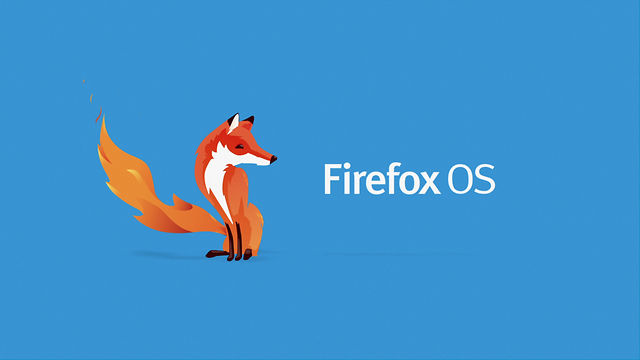
\includegraphics[scale=0.2]{./images/firefox-os.jpg}
		\\	
	\CcGroupByNcSa{0.83}{0.95ex}\\[2.5ex]
		{\tiny\CcNote{\CcLongnameByNcSa}}
		\vspace*{-2.5ex}
	\end{center}
\end{frame}

\begin{frame}
\frametitle{
\includegraphics[scale=0.4]{./images/Genma.jpg} \ \ \  A propos de moi  }
\begin{columns}[c] 
\column{.55\textwidth} 
\textbf{Où me trouver sur Internet?}
\begin{itemize}
\item Le Blog de Genma : http://genma.free.fr
\item Twitter : http://twitter.com/genma
\end{itemize}
\textbf{Mes centres d'intérêts?}
\\ Plein de choses dont:
\begin{itemize}
\item Firefox OS
\end{itemize}

\column{.5\textwidth} 

\includegraphics[width=5cm,height=5cm]{./images/blog.png} 
\end{columns}
\end{frame}

%----------------------------------------------------------------------------------------
\begin{frame}
\frametitle{Remerciements}
\justifying{
Je remercie la communauté francophone autour de Firefox OS pour les builds communautaires
\url{http://builds.firefoxos.mozfr.org/}
le support, les billets de blog, la promotion de FFOS.\\
Ainsi que Mozilla pour avoir lancé FFOS.
}
\end{frame}
%----------------------------------------------------------------------------------------
\begin{frame}
\begin{center}
\Huge{Introduction}
\\~\\
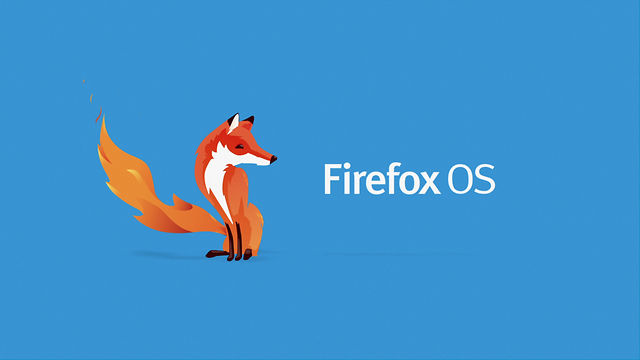
\includegraphics[scale=0.3]{./images/firefox-os.jpg}
\end{center}
\end{frame}

\begin{frame}
\frametitle{Mozilla - De Firefox à FirefoxOS}
En 2004, Mozilla a lancé Firefox, le navigateur web gratuit et
désintéressé pour votre ordinateur.
\\~\\
En 2014, Mozilla introduit en France Firefox OS, le système d’
exploitation respectueux de votre vie privée pour votre téléphone.
\end{frame}
%---------------------------------------------------------------------------------------
\begin{frame}
\frametitle{FirefoxOS - un OS libre}
Firefox OS est conçus par une communauté internationale de bénévoles, et de développeurs situés dans plusieurs pays, notamment dans les bureaux de Mozilla Paris.
\\~\\
Le logiciel est libre : Firefox OS est un logiciel libre, sans secrets, auditable. Tout le code source est ouvert et disponible.
\end{frame}
%---------------------------------------------------------------------------------------
\begin{frame}
\frametitle{Architecture de FFOS}
\begin{center}
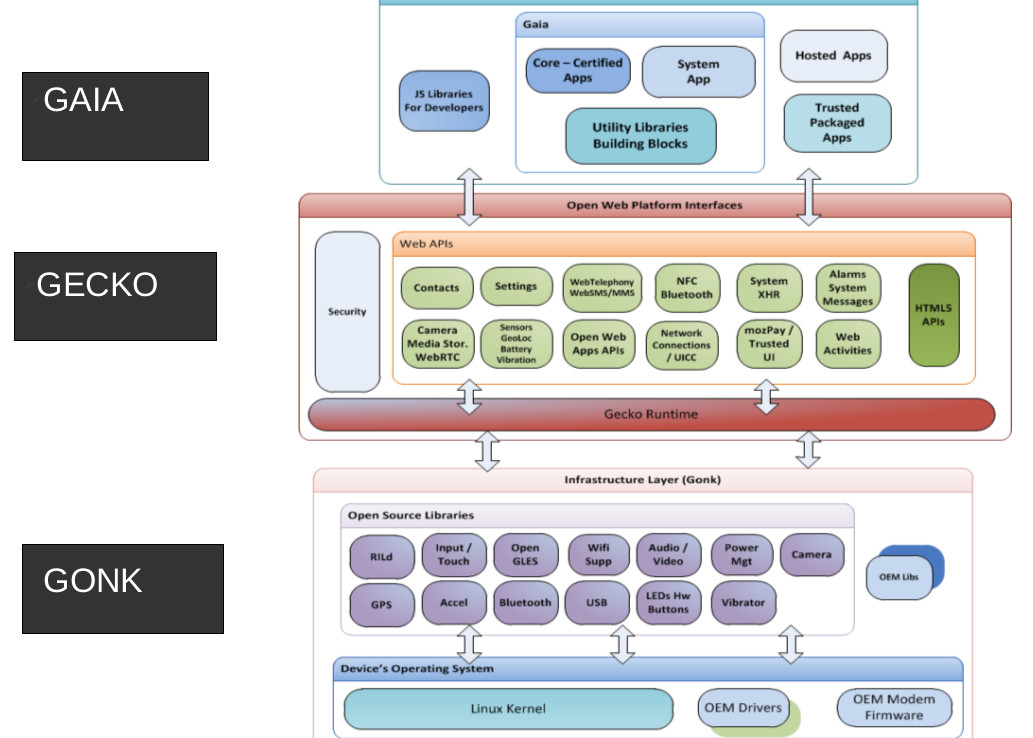
\includegraphics[scale=0.3]{./images/ffos_architecture.jpg}
\end{center}
\end{frame}

\begin{frame}
\begin{center}
\includegraphics[scale=0.06]{./images/Firefox_Layers.jpg}
\end{center}
\end{frame}
%---------------------------------------------------------------------------------------
\begin{frame}
\frametitle{Architecture de FFOS}
\begin{block}{Gaia - l'interface}
\justifying{Gaia a le rôle d'interface utilisateur de Firefox OS et contrôle tout ce qui interagit avec l'écran.}
\end{block}
\begin{block}{Gecko - le moteur}
\justifying{
Gecko est l'application permettant d'exécuter Firefox OS. Il permet le support  des trois standards : HTML, CSS et JavaScript.}
\end{block}
\begin{block}{Gonk - le noyau}
\justifying{Gonk consiste en un noyau Linux et une couche d'abstraction matérielle de l'espace utilisateur (HAL).}
\end{block}
\end{frame}


%----------------------------------------------------------------------------------------
\begin{frame}
\begin{center}
\Huge{Quel matériel?}
\\~\\
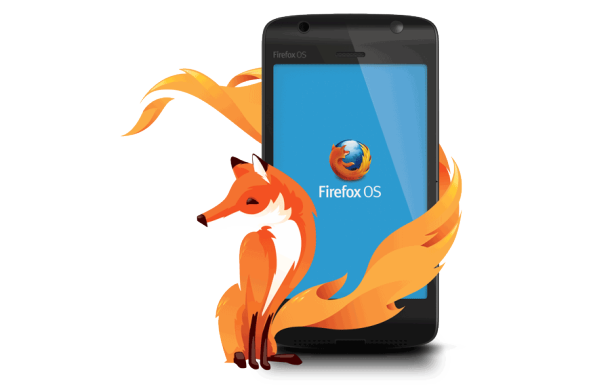
\includegraphics[scale=0.3]{./images/FirefoxOS-logo_610x385.png}
\end{center}
\end{frame}

\begin{frame}
\frametitle{Les smartphones existants}
\justifying{
En décembre 2014, on dénombre 14 opérateurs qui commercialisent dans 28 pays à travers le monde des téléphones ayant comme système d'exploitation Firefox OS.}
\begin{itemize}
\item Le ZTE Open C
\item Le Flame
\item Autres téléphones...
\end{itemize}
\begin{center}
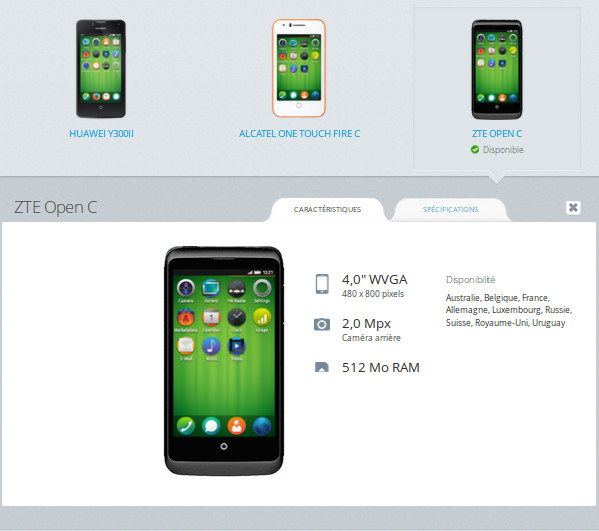
\includegraphics[scale=0.3]{./images/smartphone01.jpg}
\end{center}
\end{frame}

\begin{frame}
\frametitle{Les smartphones qui vont arrivés sur le marché}
\begin{itemize}
\item Le ZTE Open L
\item LG Fx0
\item Et d'autres...
\end{itemize}
\begin{center}
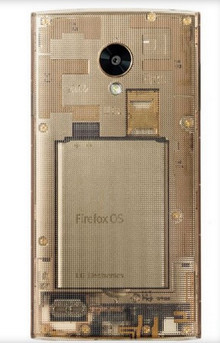
\includegraphics[scale=0.5]{./images/ffos_lg.jpg}
~~~
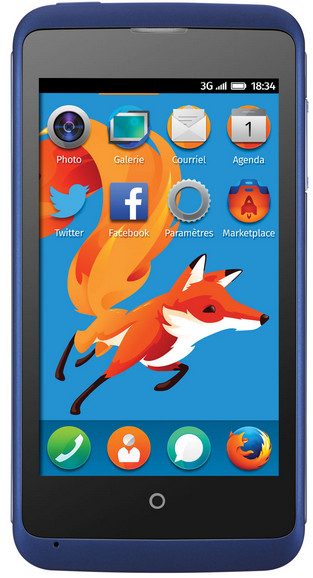
\includegraphics[scale=0.3]{./images/ZE_Open_C.jpg}
\end{center}
\end{frame}

\begin{frame}
\frametitle{Les smartphones compatibles}
\justifying{
Firefox OS est compatible avec un nombre important d'appareils, comme par exemple le Samsung Nexus S, le Samsung Nexus S 4G, le Samsung Galaxy S II, le Samsung Galaxy Nexus, le Nexus 4 et d'autres.}
\end{frame}

%----------------------------------------------------------------------------------------
\begin{frame}
\begin{center}
\Huge{Quelles appplications?}
\\~\\

\includegraphics[scale=0.3]{./images/logo_marketplace.png}
\end{center}
\end{frame}

\begin{frame}
\frametitle{Les applications par défaut dans FFOS}
\begin{columns}[c] 
\column{.55\textwidth} 
\begin{block}{Les fonctionnalités d'un smartphone}
\begin{itemize}
\item Téléphone
\item Contacts
\item SMS/MMS
\item Agenda
\item Mail
\item Firefox comme navigateur
\item ...
\end{itemize}
\end{block}
\column{.5\textwidth} 
\begin{center}
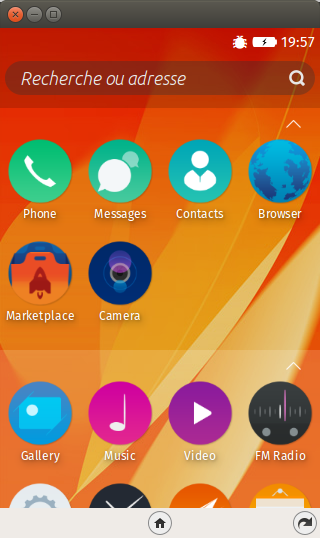
\includegraphics[scale=0.45]{./images/capture.png} 
\end{center}
\end{columns}
\end{frame}

\begin{frame}
\frametitle{Les appplications pour FFOS}
Les applications sont toutes en HTML5/CSS3/Javascript
\begin{itemize}
\item N'importe qui peut en développer une.
\item Toutes ne sont pas libres.
\end{itemize}

\begin{center}
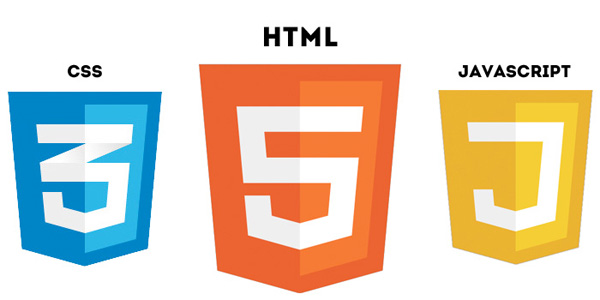
\includegraphics[scale=0.3]{./images/logo-html5.jpg} 
\end{center}
\end{frame}

\begin{frame}
\frametitle{Le marketplace}
\begin{center}
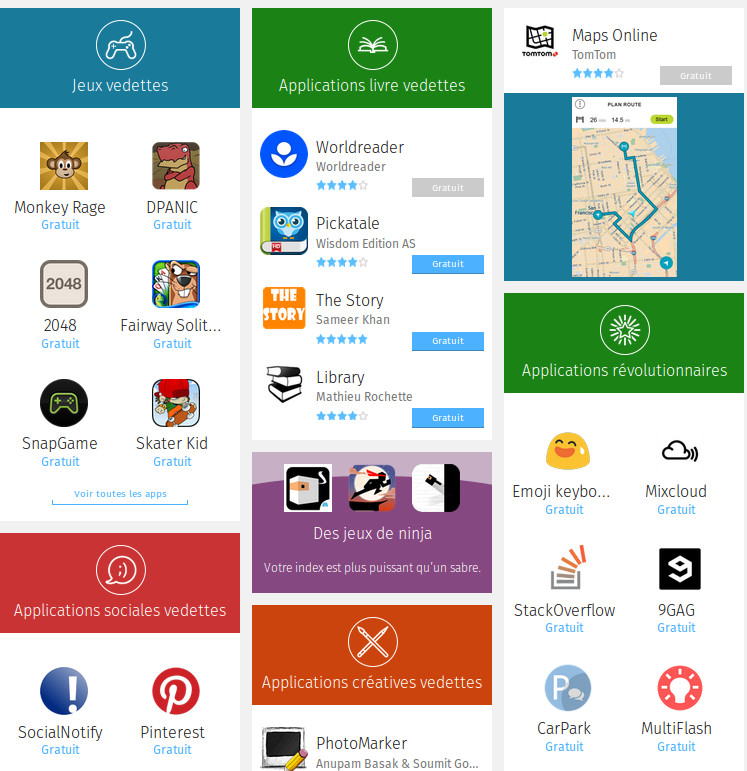
\includegraphics[scale=0.3]{./images/marketplace01.jpg}
\end{center}
\end{frame}

\begin{frame}
\frametitle{Les applications - Mon usage}
\begin{columns}[c] 
\column{.55\textwidth} 
\begin{itemize}
\item Téléphone (Appel/SMS)
\item Mail
\item Agenda
\item Twitter/Diaspora
\item Lecteur RSS
\item Consultation de site version mobile
\end{itemize}
Une sorte de mini-tablette, pour un usage ponctuel.
\column{.5\textwidth} 
\begin{center}
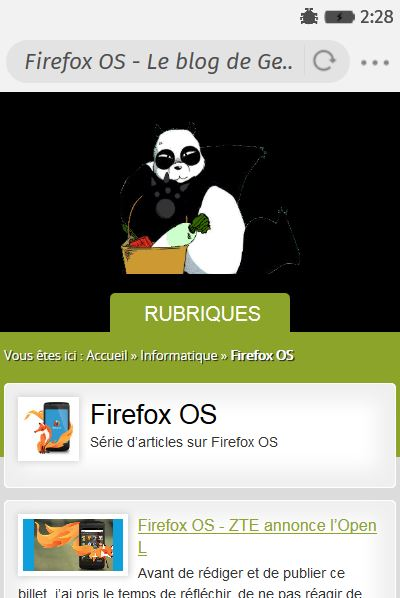
\includegraphics[scale=0.6]{./images/site_version_mobile.jpg} 
\end{center}
\end{columns}
\end{frame}
\begin{frame}
\frametitle{Les permissions des applications}
\begin{center}
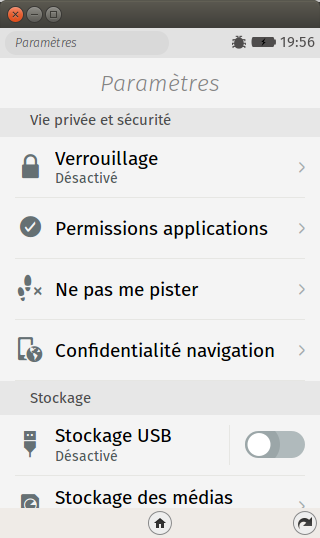
\includegraphics[scale=0.3]{./images/Screenshot01.png}
\end{center}
\end{frame}
%----------------------------------------------------------------------------------------
\begin{frame}
\begin{center}
\Huge{Où trouver des informations \\ sur FFOS?}
\end{center}
\end{frame}
\begin{frame}
\frametitle{Où trouver des informations sur FFOS?}
\begin{itemize}
\item Le site officiel par Mozilla \url{https://www.mozilla.org/fr/firefox/os/}
\item Le forum de Mozilla-fr \url{https://forums.mozfr.org}
\item Les mailing-listes \url{http://mozfr.org/participer}
\item Bugzilla \url{https://bugzilla.mozilla.org}
\item Les blogs de la communauté \url{http://mozfr.org}
\item Twitter/Diaspora-Framasphère via \#FirefoxOS
\end{itemize}
\end{frame}

%----------------------------------------------------------------------------------------
\begin{frame}
\begin{center}
\Huge{Les builds communautaires}
\\~\\
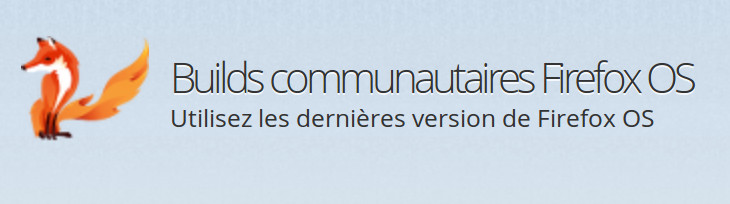
\includegraphics[scale=0.3]{./images/builds_communautaire_logo.jpg}
\end{center}
\end{frame}
%---------------------------------------------------------------------------------------
\begin{frame}
\frametitle{Les builds communautaires de FirefoxOS}
\begin{center}
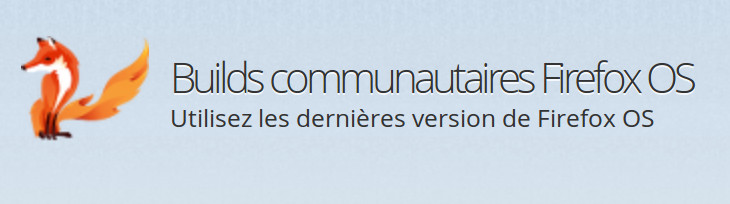
\includegraphics[scale=0.3]{./images/builds_communautaire_logo.jpg}
\\~\\
\url{http://builds.firefoxos.mozfr.org/}
\\~\\
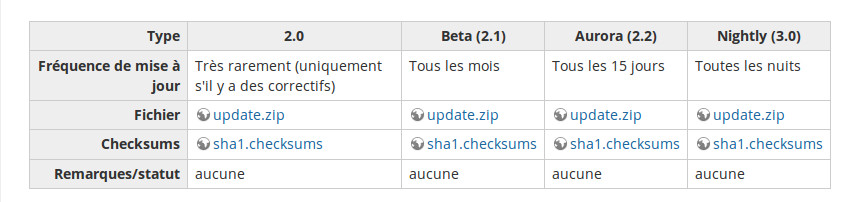
\includegraphics[scale=0.3]{./images/builds_communautaire_01.jpg}
\end{center}
\end{frame}
%---------------------------------------------------------------------------------------

\begin{frame}
\frametitle{Les builds communautaires de FirefoxOS}

\justifying{Comme le code est ouvert/disponible, la communauté construit des builds (des ROMS).}

\begin{block}{Différentes branches}
\begin{itemize}
\item Beta : 2.1
\item Aurora : 2.2
\item Nighty Build : 3.0
\end{itemize}
\end{block}

\begin{block}{Les avantages des buils communautaires}
\justifying{
\begin{itemize}
\item Relativement stable
\item Communauté réactive et sympathique. 
\item Permet d'avoir des fonctionnalités plus évoluées que la ROM par défaut.
\end{itemize}}
\end{block}
\end{frame}
%----------------------------------------------------------------------------------------
\begin{frame}
\begin{center}
\Huge{Tester FFOS?}
\\~\\
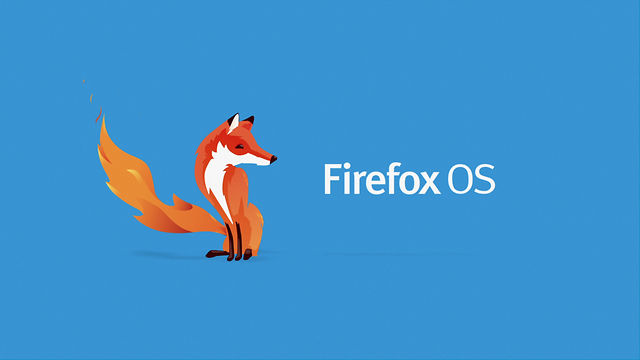
\includegraphics[scale=0.3]{./images/firefox-os.jpg}
\end{center}
\end{frame}
%----------------------------------------------------------------------------------------
\begin{frame}
\frametitle{Tester FFOS}
Le simulateur de FFOS dans Firefox le navigateur. 

\begin{center}
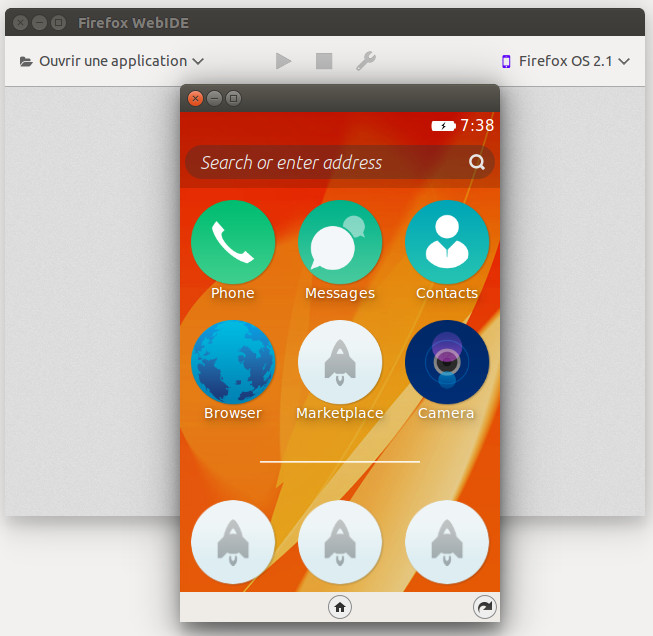
\includegraphics[scale=0.3]{./images/ffos_simulator.jpg}
\end{center}
\justifying{
Une fois l'extension installée, Menu Outil>Développement web >Web ide (MAJ+F8).
Cela donne un aperçu de ce qu'est FirefoxOS.
}
\end{frame}

%----------------------------------------------------------------------------------------
\begin{frame}
\begin{center}
\Huge{Passer à FFOS ou attendre?}
\\~\\
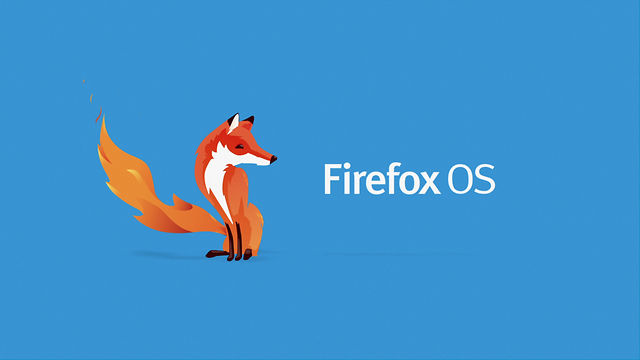
\includegraphics[scale=0.3]{./images/firefox-os.jpg}
\end{center}
\end{frame}
%----------------------------------------------------------------------------------------

\begin{frame}
\frametitle{Passer à FFOS ou attendre?}
\begin{block}{Si on est Android/IOS addict}
\justifying{
NON. Car il y aura l'application indispensable dont on ne peut se passer...
}
\end{block}

\begin{block}{Geek curieux, libriste ou 1er Smartphone}
\justifying{
Oui, mais avec un build communautaire.
}
\end{block}

\begin{block}{Ce qu'il me manque dans FFOS}
\justifying{
\begin{itemize}
\item Le chiffrement du stockage (SD-Card)
\item Des applications comme Texte-Secure...
\item Le TorBrowser
\item La connexion via un VPN
\end{itemize}
}
\end{block}
\end{frame}

%----------------------------------------------------------------------------------------
\begin{frame}
\begin{center}
\Huge{FFOS Bilan}
\\~\\
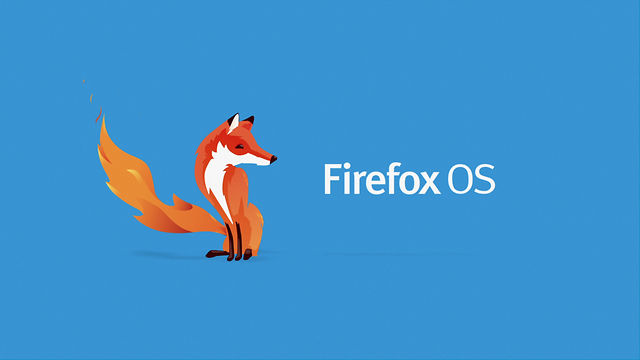
\includegraphics[scale=0.3]{./images/firefox-os.jpg}
\end{center}
\end{frame}
%----------------------------------------------------------------------------------------

\begin{frame}
\frametitle{FFOS Bilan}
\begin{block}{Les plus}
\justifying{
\begin{itemize}
\item C'est le système le plus libre, le plus ouvert et le seul à n'être pas développé par une entreprise commerciale.
\item Les builds communautaires
\item OS libre
\item TOUT EST WEB (HTML5/CSS3/Javascript)
\end{itemize}
}
\end{block}

\begin{block}{Les moins}
\justifying{
\begin{itemize}
\item OS jeune (bugs, manque de fonctionnalités)
\item Constructeurs frileux
\item Pas de smartphone haut de gamme
\end{itemize}
}
\end{block}
\end{frame}

%---------------------------------------------------------------------------------------

\begin{frame}
\begin{center}
\Huge{Questions et discussion}
\\~\\
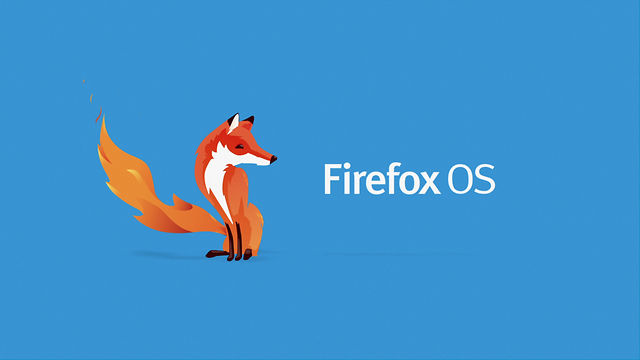
\includegraphics[scale=0.3]{./images/firefox-os.jpg}
\end{center}
\end{frame}
%----------------------------------------------------------------------------------------
\end{document}
